\documentclass[../main.tex]{subfiles}
\begin{document}
\chapter{Testing del software e di servizi}
\section{Introduzione}
\paragraph{}La diffusione del cloud computing ha portato negli ultimi anni a un cambiamento delle modalità di utilizzo del software. Esso viene fornito as-a-service; ecco dunque che l'affidabilità dello stesso assume un ruolo critico in relazione all'evoluzione scientifico-tecnologica che si sta configurando nel mondo dell'ITC.\newline
\paragraph{}
Il collaudo del software consiste nella verifica dinamica\footnote{L'attività di testing implica l'esecuzione del programma sui dati in input valutati. Il solo valore dell'input non è sufficiente per determinare un test.} del comportamento di un programma su un set finito\footnote{Anche per i programmi semplici sono teoricamente applicabili un'infinità di casi di test nel testing esaustivo e ciò implica che l'esecuzione potrebbe durare anche anni.} di casi di test, scelti in modo appropriato da un dominio di esecuzioni infinite, contro il comportamento atteso\footnote{Deve essere possibile decidere se i risultati osservati dall'esecuzione di un programma sono accettabili o no, altrimenti il collaudo è inutile} specificato \cite{AntoniaBertolino03}.
\paragraph{}
La separazione concettuale tra attività di debugging e attività di testing fu introdotta da Glenford J. Myers nel 1979 \cite{ArtOfSwTesting}, che ha illustrato il desiderio della comunità ingegneristica di dividere il processo di development - e debugging - da quello di verifica.
Gelperin e Hetzel \cite{GrowthOfSwTesting} hanno poi classificato le fasi (nel 1988) e gli obiettivi del testing individuando i seguenti periodi:
\begin{itemize}
\item Fino al 1956 - Collaudo orientato al debugging
\item 1957-1978 - Collaudo orientato alla dimostrazione
\item 1979-1982 - Collaudo orientato alla distruzione ("un test di successo è quello che individua almeno un bug" \cite{ArtOfSwTesting}
\item 1983-1987 - Collaudo orientato alla valutazione
\item 1988-2000 - Collaudo orientato alla prevenzione
\end{itemize}
A queste fasi ne va poi aggiunta una sesta, che costituisce l'obiettivo principale del progetto CUMULUS nel quale si inserisce il presente elaborato di tesi: collaudo orientato alla certificazione di servizi cloud.
Quest'ultima fase verrà discussa nei capitoli a seguire.
\section{Aspetti economici}
Il NIST\footnote{National Institute of Standard - \textit{http://www.nist.gov}} ha effettuato una stima dei costi aggiuntivi provocati dalle vulnerabilità software dovute all'inadeguatezza della strutture di testing: essi si aggirano tra i 22 e i 59 miliardi di dollari. Più della metà di questa cifra è sostenuta dagli utenti finali in termini di mitigazione e strategie di contenimento dell'errore, mentre la parte rimanente è sostenuta dagli sviluppatori e riflette le spese aggiuntive causate dall'utilizzo di strumenti e metodi di test inadeguati \cite{NistEconomicImpact}. Un influsso positivo è stato tuttavia dato dall'avvento delle moderne pratiche di deployment continuativo e dei servizi cloud, che hanno notevolmente ridimensionato i costi di re-installazione e patching dei prodotti.\newline
L'attività di collaudo diventa perciò di fondamentale importanza all'interno del ciclo di vita di un software. Lo scopo è quello di individuare le carenze di correttezza, completezza, affidabilità e sicurezza di un prodotto nella fase di development.
Essa non è una attività isolata, né un'attività di sviluppo. È piuttosto un'attività di supporto: insignificante se separata dai processi di sviluppo e di per se non produttiva \cite{GAST}.\newline
Non è quindi stata ancora definita come una scienza a se stante, è piuttosto un altro aspetto del processo di sviluppo \cite{ArtOfSwTesting}.
\paragraph{Attività del collaudo di software}
Le attività di collaudo del software possono quindi essere distinte in quattro fasi principali:
\begin{itemize}
\item \textbf{Generazione degli input (in numero sufficiente)}. Avviene generalmente quando è disponibile un implementazione del programma. Non è però esclusa la possibilità di generare input di test sulla base di un modello formale \cite{DickFaivre93} o manualmente \cite{XieDissertation}.
\item \textbf{Generazione degli output attesi, per un largo insieme di elementi in input}. Gli output attesi vengono generati per aiutare a determinare se il programma si comporta correttamente in modo globale o solo in una particolare esecuzione. Gli sviluppatori possono generare un output atteso per ogni test input specifico
%ELIA a livello globale, non globalmente (troppi 'mente' :D) %PATRIZIO: in modo globale va bene?
\cite{XieDissertation} \cite{Panzl78}.
\item Esecuzione del test con gli input generati (continuamente ed efficientemente) Il testing continuativo è importante per essere sicuri che cambiamenti al software non causino un malfunzionamento \cite{XieDissertation}.
\item Confronto degli output del test con gli output  attesi
\cite{XieDissertation}.
\end{itemize}
\paragraph{}
È comunemente accettata l'impossibilità di realizzare un software perfetto. È quindi necessario collaudarlo prima del rilascio, al fine di ridurre il rischio di sbagli nella produzione del software, ed evitando quindi l'impatto negativo quando il software viene usato.
Il collaudo dinamico è necessario, ma non sufficiente a fornire la sicurezza che il software si comporterà come voluto. Pertanto, è buona norma utilizzare anche altre attività statiche di supporto, come revisioni paritarie e analisi statica del codice \cite{iso29119}.
\section{Metodologie di testing}
\subsection{White box testing}
Il testing White box, anche noto come test strutturale, si occupa del collaudo delle procedure e delle strutture interne di un programma, in relazione a quanto esposto verso l'utente finale.
Affinché sia possibile eseguire un collaudo di questo genere è necessario avere capacità di programmazione e una visione globale dei componenti interni del sistema, in funzione dei quali si scelgono gli input del caso di test.
Questo approccio, sebbene possa essere applicato a tutti i livelli del processo di testing, viene generalmente utilizzato per il test unitario.
In ogni caso questo metodo di test può lasciare scoperti molti problemi e non essere efficace per il riconoscimento delle funzionalità non ancora implementate.
Le tecniche utilizzate comprendono:
\begin{itemize}
\item Testing delle APIs esposte all'esterno
\item Testing sulla copertura del codice, che può essere effettuato secondo varie metriche
\begin{itemize}
\item \textit{Function coverage}, restituisce la lista delle procedure chiamate.
\item \textit{Statement coverage}, restituisce il numero di linee di codice eseguite per completare il test.
\item \textit{Decision coverage}, restituisce i valori boolean per ogni ramo del diagramma di flusso durante l'esecuzione di un test.
\end{itemize}
\item Inserimento volontario di errori
\item Testing statico del codice
\end{itemize}
\subsection{Black box testing}
Questo approccio consiste nel considerare il software come una scatola nera.
Il tester esamina la funzionalità senza alcuna conoscenza di come essa sia stata effettivamente implementata; egli conosce solamente ciò che il software dovrebbe fare, non il modo in cui lo fa.
Spesso questo tipo di testing è categorizzato come "test di accettazione" ed è demandato all'utente finale, che il più delle volte non ha competenze di programmazione.
Può coincidere o meno con le fasi di rilascio del software:
\begin{itemize}
\item Alpha testing
\`E solitamente eseguito internamente, come test di accettazione, prima della fase di beta testing.
Consiste nella simulazione o nell'esecuzione diretta del software da parte dei potenziali utenti finali o di una squadra di tester indipendente dal team di sviluppo.
\item Beta testing
\`E la fase successiva all'Alpha testing e viene generalmente eseguito esternamente, come test di accettazione.
Consiste nel rilascio di versioni del software (beta) a un pubblico limitato esterno al team di sviluppo, affinché essi possano rilevare difetti o bug ed effettuarne il reporting.
\end{itemize}
\subsection{Grey box testing}
Consiste in una fusione di white box testing e black box testing.
Questo approccio si avvale di una conoscenza parziale dell'implementazione di una funzionalità e viene particolarmente usato nel collaudo dell'integrazione di due componenti sviluppati da programmatori diversi, che espongono le proprie APIs.
Può avvalersi o meno di tecniche di reverse-engineering totale o parziale del prodotto.
Avendo conoscenza parziale delle specifiche di implementazione, il tester può realizzare casi di test specifici per determinate vulnerabilità attese (ad es. input malformati, SQL injection, fuzzing, test di gestione delle eccezioni).
\section{Obiettivi del testing}
Gli obiettivi delle operazioni di collaudo sono quelli di fornire informazioni a proposito della qualità dell'elemento collaudato e qualunque rischio ad essa correlate, in relazione all'accuratezza qualitativa e quantitativa dell'attività di testing; ma anche di trovare difetti nell'oggetto collaudato prima del suo rilascio per l'uso e mitigarne gli effetti \cite{iso29119}.
Queste informazioni possono poi essere utilizzate al fine di:
\begin{itemize}
\item migliorare il prodotto, rimuovendo i difetti
\item migliorare le decisioni nei processi aziendali
\item evidenziare i difetti che potrebbero rimanere nascosti
\end{itemize}
\subsection{Livelli di astrazione}
\subsubsection{Testing unitario}
Il testing unitario, noto anche come test dei componenti, verifica la funzionalità di una specifica sezione di codice.
Per i linguaggi procedurali viene effettuato a livello di funzione, nella programmazione orientata agli oggetti invece viene eseguito a livello di classe. Il suo scopo, infatti, non è quello di verificare la presenza di una funzionalità del codice, quanto quello di assicurarsi che il singolo componente funzioni correttamente e in modo indipendente.
Solitamente i casi di test vengono scritti dagli stessi sviluppatori, durante la redazione del codice, per assicurarsi che la specifica funzioni come richiesto.
Una singola unità può essere associata a più casi di test, affinché sia possibile catturare il maggior numero di rami del codice.
A seconda delle richieste dell'organizzazione, il test unitario può includere tecniche di testing statiche o dinamiche, analisi del flusso dei dati, analisi delle metriche, revisioni paritarie del codice, analisi della copertura e altre tecniche di verifica.
\subsubsection{Testing di integrazione}
Il test di integrazione serve a collaudare la compatibilità delle interfacce dei vari componenti in relazione a un modello di design del software.
Il suo scopo è quello di esporre i difetti nelle interfacce e nell'interazione tra componenti integrati, affinché il software possa lavorare come un sistema.

\subsubsection{Testing del sistema}
Il testing del sistema, anche chiamato testing end-to-end, collauda un sistema nella sua integrità per verificare la compatibilità con i requisiti.
Inoltre, il testing del sistema deve assicurarsi che il programma funzioni come previsto e non distrugga o corrompa l'ambiente operativo o di altri processi, non causi danni alla memoria condivisa, non consumi o tenga in lock un numero eccessivo di risorse, non perda il controllo di eventuali sottoprocessi paralleli da esso avviati.
\subsection{Verifica e validazione}

Lo standard ISO/IEC IEEE 29119 \cite{iso29119} a cui si è fatto riferimento specifica alcune tecniche di verifica e validazione orientate al software testing, che rappresentano il \textit{core} del processo di validazione e verifica. Altri standard, come l'ISO/IEC 12207 \cite{iso12207} e l'IEEE 1012 \cite{ieee1012} trattano l'argomento in modo più approfondito.
%ELIA: cuore al posto di core. doppio spazio prima di "Altri standard". Aggiungi sintetiche descrizioni in italiano alle sigle che sono, giustamente, in inglese. %PATRIZIO: che inendi per sigle? quelle degli standard?
Il concetto di verifica e validazione corrisponde alle due domande:
\begin{itemize}
\item \textbf{Have we built the right software?} Il software implementa i requisiti in modo corretto? (\textit{Validazione})
\item \textbf{Have we built the software right?} Il software soddisfa le esigenze del committente e i requisiti di progettazione? \textit{Verifica}
In questo modo è possibile specificare in modo più preciso il significat di Verifica e Validazione.
Queste le definizioni dal documento "IEEE Standard Glossary of Software Engineering Terminology" \cite{NistGlossary}:
\end{itemize}
\begin{itemize}
\item \textit{Verifica} è la valutazione di un sistema o un componente del sistema per determinare se il prodotto di una determinata fase di sviluppo soddisfa le condizioni imposte all'inizio di tale fase.
\item \textit{Validazione} è la valutazione di un sistema o un componente del sistema durante il processo di sviluppo o alla fine dello stesso, per determinare se soddisfa i requisiti.
\end{itemize}
Queste due definizioni sono state poi rielaborate nello standard ISO9000 \cite{iso9000} nel modo seguente:
\begin{itemize}
\item \textit{Verifica} è la conferma, svolta tramite analisi corroborate dalle evidenze necessarie, che i requisiti specificati sono stati rispettati.
\item \textit{Validazione} è la conferma, svolta tramite analisi corroborate dalle evidenze necessarie, che i requisiti per un particolare utilizzo del prodotto sono stati rispettati.
\end{itemize}

L'insieme di operazioni per un accurato piano di V\&V \footnote{Verification and Validation} comprende:
\begin{itemize}
\item La generazione di un SVVP \footnote{Software Verification and Validation Plan}, il cui scopo è quello di fornire una descrizione dettagliata per la verifica e la validazione del codice e gli obiettivi dello stesso processo di validazione \cite{ieee1012}.
\item Valutazione delle modifiche alla baseline
\item Gestione e supporto alla revisione del V\&V
\end{itemize}

\subsection{Testing come euristica}
In ingegneria (e ingegneria del software), un'euristica è un metodo basato sull'esperienza che può essere usato come sostegno per rappresentare e risolvere i problemi. È più che altro utile nella creazione di modelli di sistemi da testare; potrebbe però comunque fallire nella modellazione completa del sistema e pertanto portare a un mancato rilevamento di tutti i difetti \cite{iso29119}.
%ELIA potrebbe però
\section{Testing nel contesto organizzativo di un progetto}
In ogni tipo di organizzazione produttrice di software, sia essa una multinazionale con migliaia di tester oppure una società individuale, il testing del software dovrebbe occupare un ruolo di assoluta importanza dal punto di vista dell'organizzazione del business.
Talvolta, il processo di testing può essere compiuto senza alcuna politica formalizzata e strategie organizzative, in organizzazioni di minore maturità. Questa pratica, tuttavia, fornisce meno coerenza al processo rendendolo meno effettivo e efficiente \cite{iso29119}.\paragraph{}
Il processo di collaudo è strettamente legato al contesto in cui si svolge. Ciò significa che deve essere pianificato, monitorato e controllato.
Il contesto può essere un progetto in sviluppo o la manutenzione continuativa di un sistema in produzione. L'esperienza dell'industria suggerisce che non esiste alcuna strategia, piano, metodo di test funzionale per tutte le circostanze.
Il collaudo di un progetto viene spesso suddiviso in un numero di sottoprocessi: ognuno di questi ha uno specifico Test Plan, consistente di una strategia di sottoprocesso allineata alla strategia globale del progetto \cite{iso29119}.
\begin{figure}[H]
\centering
\makebox[\textwidth]{
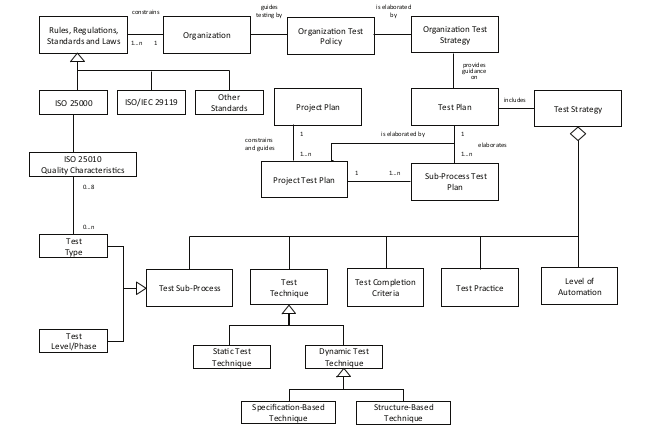
\includegraphics[width=13cm]{immagini/iso29119_fig1.png}
}
\caption{Test in un contesto multi-layer - ISO29119 \cite{iso29119}}\label{fig:2}
\end{figure}
La Figura \ref{fig:2} mostra chiaramente come il testing si inserisce in un contesto aziendale stratificato.
Il contesto è composto da leggi, regolamenti e standard industriali, intersecate con le politiche e le procedure sviluppate dall'organizzazione stessa per rendere efficiente l'attività di testing.
Ogni processo può essere indirizzato a più di un livello di test (per esempio, il piano di test di sicurezza si sviluppa ortogonalmente rispetto ai vari livelli di test funzionali).
Le strategie di testing, inoltre, descrivono anche la modalità con cui i test vengono eseguiti \cite{iso29119}.
%ELIA: la figura 2.2, non 1.2! idem la 2.3, al posto di 1.3, più sotto :)
\begin{figure}[H]
\centering
\makebox[\textwidth]{
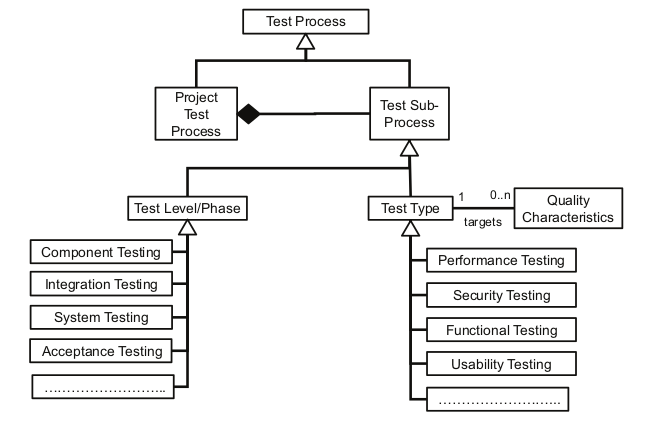
\includegraphics[width=15cm]{immagini/iso29119_fig2.png}
}
\caption{Relazione tra i sottoprocessi, i livelli e i tipi di test - ISO29119 \cite{iso29119}}\label{fig:3}
\end{figure}
La Figura \ref{fig:3} descrive la relazione tra il processo di test generico, il sottoprocesso di test generico, i livelli e i vari tipi di test.
Il sottoprocesso può essere quindi eseguito nei seguenti modi:
\begin{itemize}
\item Come un livello o una fase di test
\item Come un tipo di test
\item Un sottoprocesso associato a un determinato livello può incapsulare altri sottoprocessi
\item I sottoprocessi che compongono il processo di test relativo a tutto il progetto possono essere messi in sequenza (test del progetto = test dei componenti + test di integrazione + test del sistema + test di accettazione)
\end{itemize}
Inoltre viene meglio descritta la relazione tra i tipi di test e le caratteristiche qualitative (per come definite nella ISO/IEC 25010 (ex. ISO/IEC 9126)) \cite{iso29119}
\section{Le caratteristiche qualitative}
Lo standard ISO/IEC 25010 \cite{iso25010}, aggiornamento dello standard ISO/IEC 9126 \cite{iso9126}, divide le caratteristiche qualitative in otto categorie, come rappresentato nella figura 2.4.

\begin{figure}[H]
\centering
\makebox[\textwidth]{
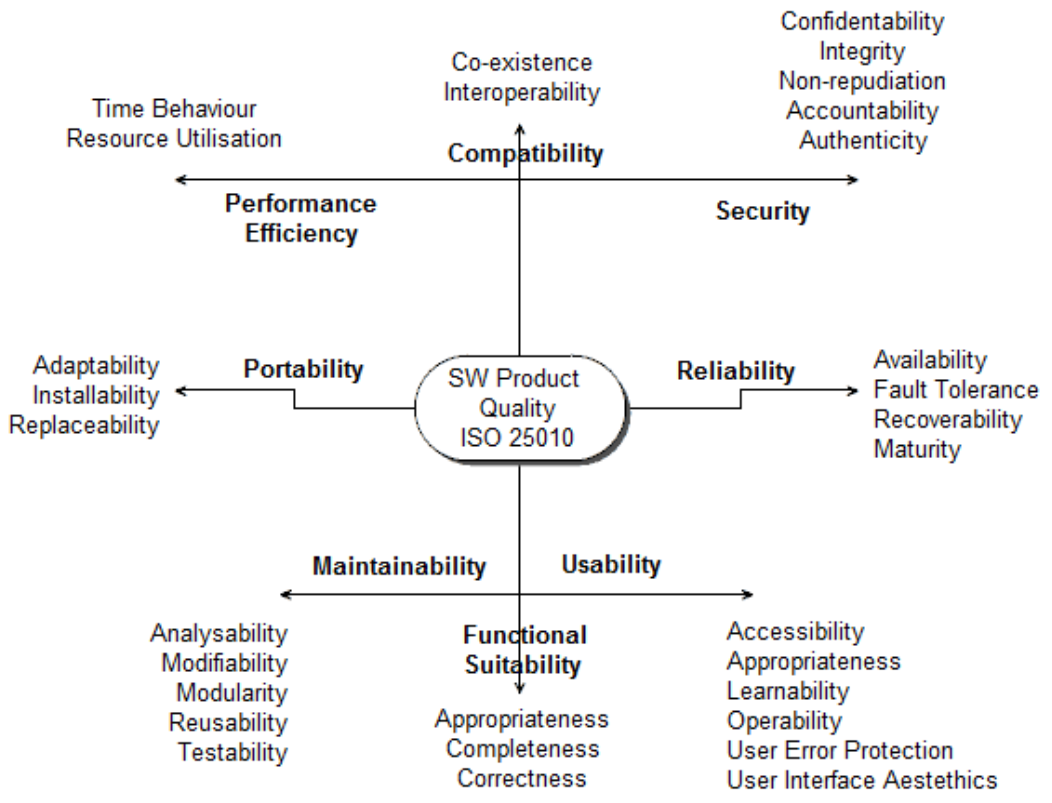
\includegraphics[width=15cm]{immagini/iso25010.png}
}
\caption{Qualità del prodotto in ISO/IEC 25010 \cite{iso25010}}\label{fig:4}
\end{figure}

\paragraph{Funzionalità}
La funzionalità è l'insieme di capacità del prodotto che stabiliscono che le proprietà implementate da un prodotto o un sistema  rispettino le esigenze effettive sotto determinate condizioni. Essa è composta dalle seguenti sotto-caratteristiche:
\begin{itemize}
\item \textbf{Completezza} - Capacità per la quale un determinato set di funzioni copre i processi specificati e gli obiettivi dell'utente
\item \textbf{Correttezza} - Capacità per la quale un prodotto o un sistema forniscono i risultati corretti con il corretto livello di precisione
\item \textbf{Appropriatezza} - Capacità per cui le funzioni facilitano il raggiungimento degli obiettivi del prodotto
\end{itemize}
\paragraph{Efficienza nelle prestazioni}
Questa caratteristica rappresenta le prestazioni in relazione al numero di risorse usate da un prodotto o un sistema, sotto determinate condizioni.
È composta dalle seguenti sotto-caratteristiche
\begin{itemize}
\item \textbf{Comportamento nel tempo} - Capacità per cui il tempo di elaborazione, il tempo di risposta e tasso di produttività corrispondano alla specifica.
\item \textbf{Utilizzo di risorse} - Capacità per la quale la somma e i tipi di risorse utilizzati da un prodotto o sistema rispetti i requisiti.
\item \textbf{Capacità} - Capacità per cui il limite massimo di un parametro all'interno del prodotto o del sistema rispetti i requisiti.
\end{itemize}

\paragraph{Compatibilità}
Questa caratteristica rappresenta le capacità di un sistema di interoperare con altri prodotti, sistemi o componenti e di eseguire le sue funzioni, condividendo con essi lo stesso ambiente hardware o software. È composta dalle seguenti sotto-caratteristiche:
\begin{itemize}
\item \textbf{Coesistenza} - Capacità per cui un prodotto può eseguire le sue funzioni basilari in modo efficiente condividendo un ambiente e delle risorse comuni con altri prodotti, senza impatti dannosi su di essi.
\item \textbf{Interoperabilità} - Capacità per cui due o più sistemi, prodotti o componenti possono scambiarsi informazioni e usare efficientemente le informazioni scambiate.
\end{itemize}

\paragraph{Usabilità}
Questa caratteristica rappresenta la capacità di un sistema, prodotto o componente di raggiungere gli obiettivi specificati in modo effettivo, con efficienza e soddisfazione nello specifico contesto. È composta dalle seguenti sotto-caratteristiche:
\begin{itemize}
\item \textbf{Riconoscimento di idoneità} - Caratteristica per cui un sistema, prodotto o componente può essere riconosciuto come idoneo per l'utilizzo dall'utente finale.
\item \textbf{Apprendibilità} - Capacità per cui un sistema, prodotto o componente può essere usato da utenti specifici per raggiungere obiettivi specifici di apprendimento all'utilizzo, in modo effettivo, efficiente, libero da rischi, soddisfacente nel contesto specifico.
\item \textbf{Operabilità} - Capacità per cui un prodotto o sistema ha attributi che lo rendano facile da controllare. 
\item \textbf{Protezione nell'utilizzo da parte dell'utente} -  Capacità di un sistema di proteggere gli utenti dal commettere errori.
\item \textbf{Estetica dell'interfaccia utente} -  Capacità di offrire un'interfaccia grafica che garantisca un'interazione con l'utente soddisfacente e gradevole.
\item \textbf{Accessibilità} -  Capacità di un sistema di essere usato da persone con un largo range di caratteristiche e capacità di raggiungere un obiettivo specifico in un contesto specifico.
\end{itemize}

\paragraph{Affidabilità}
Questa caratteristica rappresenta la capacità di un sistema, prodotto o componente di eseguire specifiche funzioni sotto specifiche condizioni per no specifico periodo di tempo. È composta dalle seguenti sotto-caratteristiche:
\begin{itemize}
\item \textbf{Maturità} - Caratteristica per cui un sistema, prodotto o componente incontra la necessità di affidabilità durante le sue normali operazioni.
\item \textbf{Disponibilità} - Capacità per cui un sistema, prodotto o componente è operativo e accessibile quando richiesto per l'uso.
\item \textbf{Tolleranza ai guasti} - Capacità per cui un sistema, prodotto o componente opera come previsto, anche in caso di danni all'hardware o al software ad esso sottostante.
\item \textbf{Recuperabilità} - Capacità per cui un sistema o prodotto, in caso di interruzione del funzionamento o guasto, può recuperare i dati coinvolti nel guasto e ristabilire il suo stato funzionale.
\end{itemize}

\paragraph{Sicurezza}
Questa caratteristica rappresenta la capacità di un sistema o prodotto di proteggere le informazioni e i dati in modo che siano disponibili solo per alcuni prodotti, sistemi o persone con diversi livelli di autorizzazione (controllo degli accessi).
È composta dalle seguenti sotto-caratteristiche
\begin{itemize}
\item \textbf{Confidenzialità} - Capacità di assicurarsi che i dati siano accessibili solo a chi è autorizzato ad accedervi.
\item \textbf{Integrità} - Capacità di prevenire l'accesso non autorizzato o la modifica di programmi o dati.
\item \textbf{Non ripudio} - Capacità di dimostrare azioni od eventi, in modo che non possano essere ripudiati successivamente.
\item \textbf{Responsabilità} - Capacità di ricondurre azioni od eventi al relativo responsabile in modo univoco.
\item \textbf{Autenticazione} - Capacità di assegnare correttamente l'identità di un soggetto o di una risorsa a chi la rivendica.
\end{itemize}


\paragraph{Manutenibilità}
Questa caratteristica rappresenta la capacità di un sistema o prodotto di essere migliorato in termini di efficienza, corretto o adattato ai cambiamenti dell'ambiente e dei requisiti.
È composta dalle seguenti sotto-caratteristiche
\begin{itemize}
\item \textbf{Modularità} - Caratteristica per cui un prodotto o sistema può essere composto di una serie discreta di componenti, in modo che il cambiamento di un singolo componente abbia un impatto minimo sugli altri. 
\item \textbf{Riusabilità} - Capacità per cui una risorsa può essere usata in uno o più sistemi o per comporre nuove risorse.
\item \textbf{Possibilità di analisi} - Possibilità di effettuare un'analisi efficiente con cui sia possibile valutare l'impatto di un cambiamento intenzionale a una o a più parti di un prodotto o sistema, o di diagnosticare le carenze di un prodotto, o di identificare le parti da modificare.
\item \textbf{Modificabilità} - Capacità di un prodotto di essere modificato effettivamente ed efficientemente senza introdurre difetti o degradarne la qualità.
\item \textbf{Possibilità di collaudo} - Capacità di un prodotto attraverso la quale è possibile stabilire un criterio di collaudo su un sistema, prodotto o componente e di stabilire se questo criterio viene rispettato.
\end{itemize}
\paragraph{Portabilità}
Questa caratteristica rappresenta la capacità di un sistema, prodotto o componente di essere trasferito da un ambiente operazionale ad un altro.
È composta dalle seguenti sotto-caratteristiche:
\begin{itemize}
\item \textbf{Possibilità di adattamento} - Capacità di un prodotto o sistema di essere adattato in modo efficiente ed effettivo ad ambienti differenti o miglioramenti hardware, software o altri aggiornamenti nell'ambiente operativo.
\item \textbf{Possibilità di installazione} - Capacità per cui un prodotto può essere efficientemente installato o disinstallato in uno specifico ambiente.
\item \textbf{Possibilità di sostituzione} - Possibilità di un prodotto di essere sostituito da un altro studiato per lo stesso scopo nello stesso ambiente.
\end{itemize}

\section{Testing basato sulle caratteristiche qualitative}
Prima di effettuare il collaudo di una qualità, è necessario instanziare un sottoprocesso di test. Ad esempio, la pianificazione di un test orientato alla misurazione delle qualità di sicurezza e la sua esecuzione potrebbe richiedere l'implementazione di un sottoprocesso di test dedicato.
Ciascuna di queste caratteristiche qualitative ha un numero di sotto-caratteristiche che possono essere collaudate per fornire una visione globale delle caratteristiche stesse. Bisogna anche ricordare che non tutte le caratteristiche sono applicabili a tutti i sistemi (es. la portabilità potrebbe non essere importante per un sistema embedded).
%ELIA integrato per embedded? %nein non si capisce "sistema integrato", anche se è un inglesismo embedded è piu specifico
Comunemente viene indicato come "collaudo funzionale" il testing applicato alle qualità funzionali (completezza, correttezza, appropriatezza). Tutte le altre qualità fanno parte del "collaudo non-funzionale" e includono tipologie di test come stress testing, penetration testing, test sul carico e sull'usabilità \cite{iso29119}.
%ELIA footnote o approfondimento su queste tipologie? 
%pat del penetration parlo più in giu... magari metto qualche footnote poi, mo vedo

\section{Testing su infrastrutture distribuite}
Parlando del collaudo dei sistemi distribuiti dobbiamo affrontare la problematica della dualità della loro natura. Bisogna dunque fare una suddivisione tra \textit{sistemi basati sul software} e \textit{sistemi semplici}\cite{disttest}.
D'altra parte però, il carattere distribuito di questi sistemi ci porta a dare importanza anche alla parte di connettività. Per questo motivo, il test delle applicazioni deve essere molto flessibile per garantire una copertura appropriata di questi sistemi e collaudare aspetti differenti con una grande varietà di requisiti \cite{disttestDelGado}.
%ELIA connettività per networking
%pat ma non te piace proprio la terminologia inglese? xD
Fortunatamente il divario che per molti anni ha caratterizzato il rapporto tra l'attività sistemistica, di sviluppo e di rete (e tra le varie figure professionali coinvolte, a causa della notevole varietà di paradigmi implicati) si sta appiattendo a causa di alcuni cambiamenti significativi:
\begin{itemize}
\item L'avvento della virtualizzazione e delle tecnologie cloud
\item L'utilizzo di tecnologie IT in ambienti di business (come quello industriale) già standardizzati
\end{itemize}
Ciò nonostante, bisogna comunque trattare l'attività di testing degli ambienti distribuiti separando i tre aspetti che questi coinvolgono \cite{disttest}.
\subsection{Testing della rete}
Le revisioni correnti dello standard ISO/IEC 9646 \cite{iso9646} e dello standard ITU-T Z.500 \cite{itutz500} definiscono i sistemi distribuiti come processi interconnessi, di conseguenza occorre effettuare un test di conformità. Il test di conformità costituisce uno strumento potente per il testing dei protocolli di rete, ma non copre completamente tutte le funzionalità di rete \cite{tretmans}.
Come descritto dall'articolo "A Formal Approach to Network/Distributed Systems Complex Testing" \cite{disttest}, una metodologia complementare a quanto descritto nello standard ISO/IEC 9646:1994 è stata data da Grabowski e Walter \cite{disttestWalterGrabowski1} \cite{disttestWalterGrabowski2} ed include le seguenti procedure:
\begin{itemize}
\item Test di conformità
\item Test di interoperabilità
\item Test funzionale
\item Test prestazionale
\end{itemize}
\subsection{Testing del software e del sistema}
In riferimento all'articolo \cite{disttest}, a quanto già scritto nel capitolo e in base agli standard IEEE 1012 \cite{ieee1012}, ISO/IEC/IEEE 12207 \cite{iso12207}, ISO/IEC/IEEE 15288 \cite{iso15288} e ISO/IEC/IEEE 29119 \cite{iso29119} andiamo ora a descrivere il testing di software e di sistema in ambienti distribuiti.
I processi tecnici di base sono i due già descritti, parlando del V\&V:
\begin{itemize}
\item Testing di accettazione del software e del sistema (processo di validazione)
\item Testing di qualificazione del software e del sistema (processo di verifica)
\end{itemize}
Mentre il testing tradizionale del software si concentra più sulla parte di code-testing e si evolve col testing di architetture distribuite e Web Services, il testing delle SOA\footnote{Service Oriented Architecture - Architettura orientata alla fornitura di servizi} si sofferma principalmente sulla logica di business \cite{disttestSoaTest1} ad esse legata. Tuttavia, ad alto livello, il collaudo di un'architettura orientata alla fornitura di servizi non differisce molto dal collaudo di un sistema distribuito tradizionale.
Specificatamente il collaudo di una SOA deve essere improntato più sulle funzionalità (prestazioni comprese) e sulla conformità degli attributi non funzionali (inclusa l'interoperabilità) \cite{disttestSoaTest2}.
%ELIA prestazioni per performances, sotto non è necessario, va bene così com'è, a condizione che usi il singolare (niente 's' finale)
\subsection{Testing delle performance}
Uno degli aspetti più importanti da collaudare in un sistema distribuito è quello prestazionale.
Le caratteristiche di performance di un'architettura distribuita sono la più importante fonte di informazioni sulle condizioni del sistema stesso, da cui il cliente potrà trarre decisioni di business \cite{disttest}.
Inoltre, il collaudo delle prestazioni costituisce uno dei fattori chiave per la valutazione dell'affidabilità del sistema.
Gli standard RFC2544 \cite{rfc2544}, RFC2889 \cite{rfc2889}, RFC3511 \cite{rfc3511} e RFC5180 \cite{rfc5180} definiscono le metodologie di benchmarking e le relative caratteristiche prestazionali \cite{disttest}.
%ELIA footnote su benchmarking %ok poi me invento qualcosa
Un approccio pratico effettivo alle attività di collaudo delle performance è descritto da R.Jain \cite{disttestJain}:
\begin{itemize}
\item Test di risorse servite per unità di tempo
\item Test del tempo di risposta
\item Test del throughput / larghezza di banda
%ELIA footnote sul termine throughput, oppure scrivi produttività. In alternativa, metti una footnote al paragrafo 121 %ok poi vedo
\item Test di utilizzo
\item Test di affidabilità (assenza di errori)
\item Test di disponibilità (uptime e downtime)
\end{itemize}

\subsection{Testing di sicurezza e penetration testing}
Un ulteriore aspetto da collaudare, soprattutto per quanto riguarda i sistemi distribuiti, cloud o semplicemente basati sulla rete, è quello della sicurezza.
Un fallimento in questo ambito potrebbe comportare un incidente informatico, andando ad impattare anche sull'economia a cui un progetto è legato.
Senza dubbio, in un ottica di cloud-computing, una delle tematiche più sentite è quella della privatezza del dato. Bisogna convincere il cliente (e, in casi estremi, una giuria), che un sistema funzioni come previsto, anche dal punto di vista della sicurezza.
I requisiti principali per le metodologie di test di sicurezza su infrastrutture distribuite e reti sono stati descritti negli standard ITU-T X 1051 \cite{disttestITUTX1051}, ISO/IEC 27001 \cite{iso27001}, ISO/IEC 27002 \cite{iso27002}, ISO/IEC 27005 \cite{iso27005}, i quali definiscono informazioni pratiche per effettuare l'analisi e la gestione dei rischi connessi alle infrastrutture distribuite.
Le implementazioni di questi standard si basano sia sui metodi formali che sull'esperienza pratica. Il testing deve essere effettuato sia sui singoli componenti del sistema che sull'ambiente preso nella sua interezza.
Il processo tecnico di base per i test di sicurezza è chiamato "penetration testing".
Varie metodologie per la valutazione della sicurezza delle infrastrutture distribuite nella loro interezza, mediante la sono stati descritti da Yong e Aitel, Allen, Weidman e altri, che forniscono un approccio basato sulla generazione e l'esecuzione automatizzata di attacchi \cite{disttest}.
\end{document}